\subsection{Others Tab}

\begin{figure}[H]
   \centering
    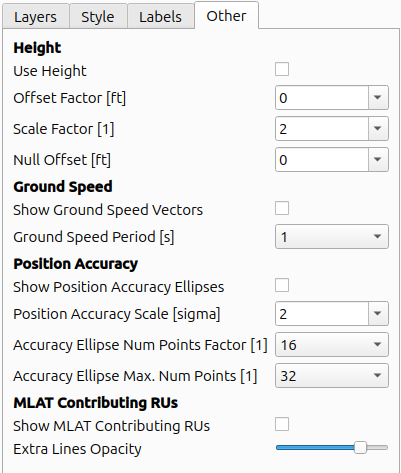
\includegraphics[width=8cm,frame]{figures/geoview_others_tab.png}
  \caption{Geographic View Others tab}
\end{figure}

In the 'Others' tab, several elements exist:

\begin{itemize}
 \item Height: Defines if and how height information is used.
 \item Ground speed: Defines if and how ground speed information is used.
 \item Position Accuracy: Defines if and how position accuracy information is used.
 \item Radar Default Accuracies: Defines Radar default accuracies.
 \item Update button: Triggers a redraw or reload of the data, becomes available after a change if needed.
\end{itemize} 

\subsubsection{Height}
\label{sec:others_height}

Per default, a target report's height is not used for display, which is common in current air-traffic displays. However, in certain situations a true 3D display might be of interest to a user, and therefore several options were incorporated:

\begin{itemize}
 \item Use Height: Use the height based on Mode C $h_c$, transformed to meters
 \item Offset Factor: If height information is used, this factor $h_o$ is added to the height
 \item Scale Factor: If height information is used, this factor $h_s$ is used to multiply the height
 \item Null Offset: If height information is used, this factor $h_n$ is used for target reports without height information
\end{itemize}
\ \\

Generally, if no height information is given (no Mode C code), the height is either $0$ or the height offset (if used). That means that those target reports appear to be on the ground. If connection lines are drawn between the ones in the air and those without, a lot of annoying lines are shown. \\

The formula to calculate the height (if existing) is as follows: 

$$ h = h_o + h_s \cdot h_c [m]$$ 

If no height information is given:

$$ h = h_n [m]$$ 


\begin{figure}[H]
    \centering
    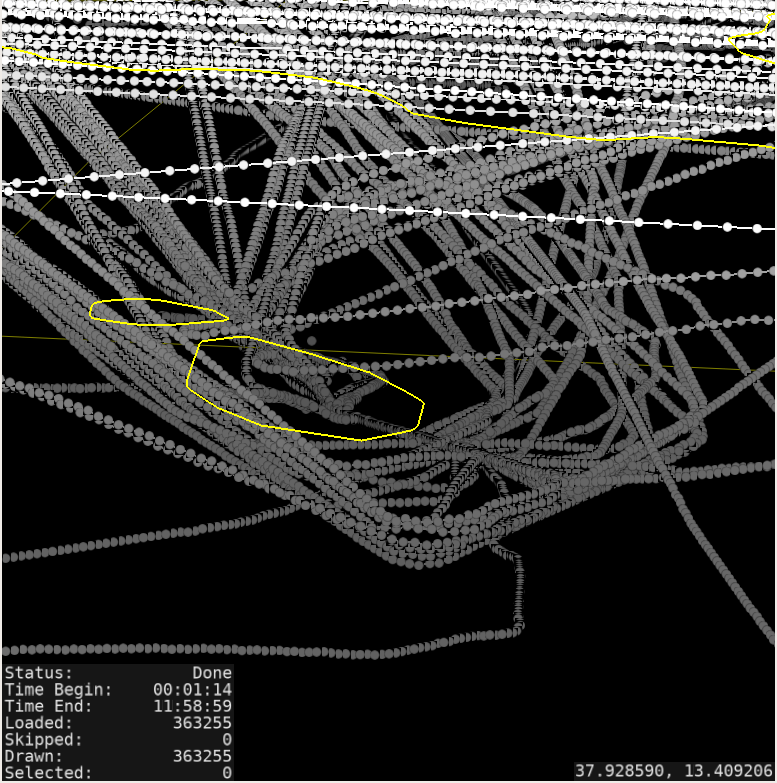
\includegraphics[width=12cm,frame]{figures/geoview_use_height.png}
  \caption{Geographic View use height}
\end{figure} 

\subsubsection{Ground Speed}
\label{sec:others_ground_speed}

\begin{itemize}
 \item Show Ground Speed Vectors: Defines if ground speed should be shown automatically for all data.
 \item Ground Speed Period [s]: Length of ground speed vectors, in seconds.
\end{itemize}
\ \\

For specific target reports the ground speed vectors can be shown using \nameref{sec:data_operations}.

\begin{figure}[H]
    \centering
    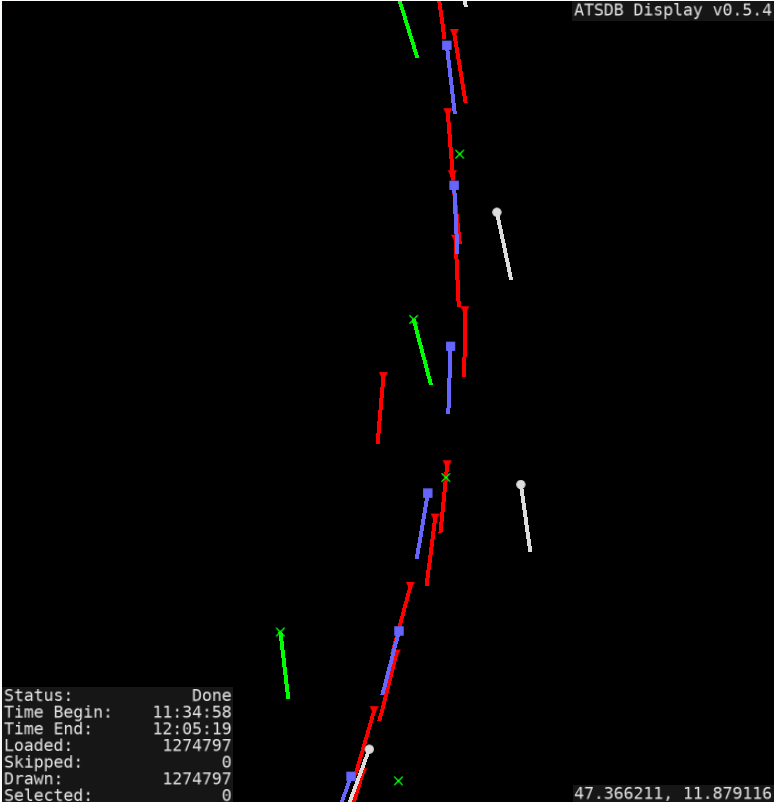
\includegraphics[width=12cm,frame]{figures/geoview_groundspeed_vectors.png}
  \caption{Geographic View ground speed vectors}
\end{figure} 


\subsubsection{Position Accuracy}
\label{sec:others_position_accuracy}

\begin{itemize}
 \item Show Position Accuracy Ellipses: Defines if Position Accuracy Ellipses should be shown automatically for all data.
 \item Position Accuracy Scale [sigma]: Size of accuracy ellipses, defined in standard deviations:
 \begin{itemize}
    \item 1.0 $\sigma$: 68.268 \%
    \item 2.0 $\sigma$: 95.44 \%
    \item 3.0 $\sigma$: 99.73 \%
    \item 4.0 $\sigma$: 99.9936 \%
    \item 5.0 $\sigma$: 99.99994266 \%
\end{itemize}  
\item Accuracy Ellipse Num Points Factor [1]: Multiplication factor to calculate number of ellipse points based on size
\item Accuracy Ellipse Max. Num Points [1]: Maximum number of ellipse points
\end{itemize}
\ \\

For specific target reports, position accuracy ellipses can be shown using \nameref{sec:data_operations}:

\begin{figure}[H]
    \centering
    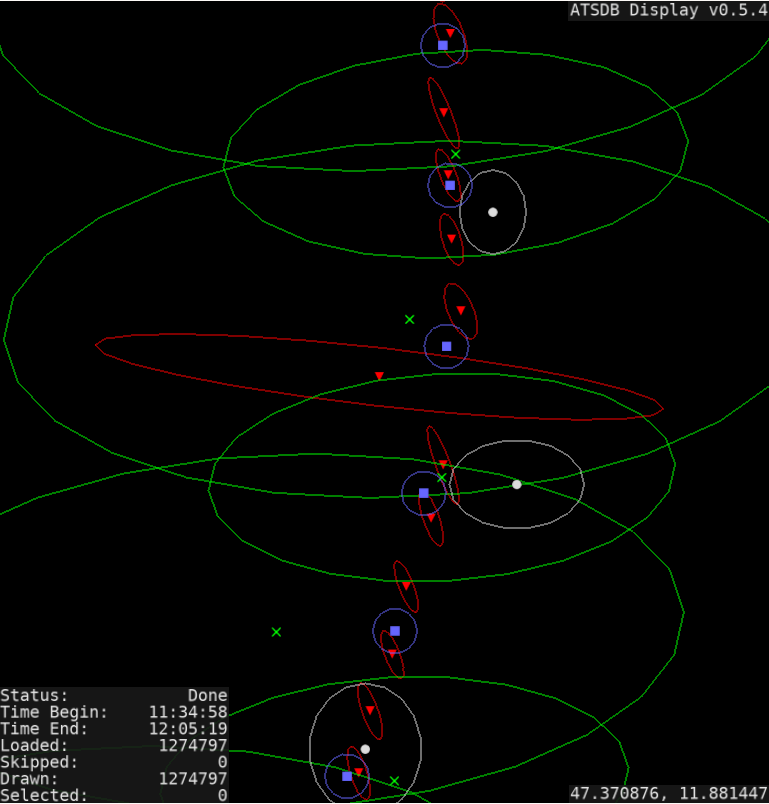
\includegraphics[width=12cm,frame]{figures/geoview_accuracy_ellipses.png}
  \caption{Geographic View position accuracy ellipses}
\end{figure} 

How the position accuracy ellipses are generated is defined in \nameref{sec:algo_position_accuracy_ellipses}.

\subsubsection{MLAT Contributing RUs}
\label{sec:others_mlat_contributing_rus}
\label{sec:geo_mlat_connection_lines}

For MLAT target reports, the Geographic View can draw connection lines from each report to its contributing Remote Units. The lines are only available where the source data contains contributing receiver information and where the parent MLAT Data Source has Remote Units defined (see \nameref{sec:ui_configure_ds_mlat_rus}). \\

The 'Others' tab provides the global toggle:

\begin{itemize}
 \item Show MLAT Contributing RUs: Enables or disables MLAT connection lines for the entire view
\end{itemize}
\ \\

The connection lines can additionally be toggled per target report or per layer / data item via the right-click context menus (see \nameref{sec:data_operations}):

\begin{itemize}
\item Per target report: 'Show MLAT Contributing RUs' / 'Clear MLAT Contributing RUs'
\item Per layer or data item (Parent UTN, Parent DBContent CAT020, Parent Root): same actions
\end{itemize}
\ \\

The context-menu actions only appear on items whose underlying data contains contributing receivers.

\begin{figure}[H]
    \centering
    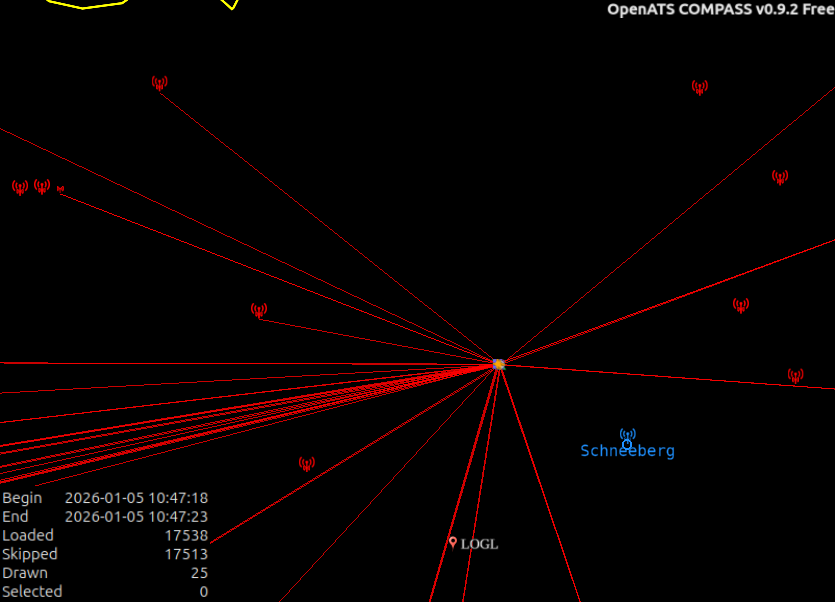
\includegraphics[width=16cm,frame]{figures/geoview_mlat_rus.png}
  \caption{Geographic View MLAT Remote Units}
\end{figure}

\subsubsection{Extra Lines Opacity}

The slider at the bottom of the 'Other' tab changes the line opacity for all optional informative lines uniformly:
\begin{itemize}
 \item Ground speed vectors
 \item Position accuracy ellipses
 \item ARTAS target report usages
 \item MLAT Contributing RUs connection lines
\end{itemize}
\ \\

Typical use:
\begin{itemize}
\item High opacity: brings fine details forward when only a few lines are visible
\item Low opacity: reveals density patterns in busy regions
\end{itemize}
\ \\


